\section{system design}
We have developed an Android application, DirectionDetector, which provides an interface for starting and stopping the detection process. The application interface displays the estimated angle and also provides a visual representation [have to add a speedometer kind of interface] of the estimated angle. Figure ~\ref{fig:screenshot} [insert a figure number here] shows the screenshot of the application.

\begin{figure}
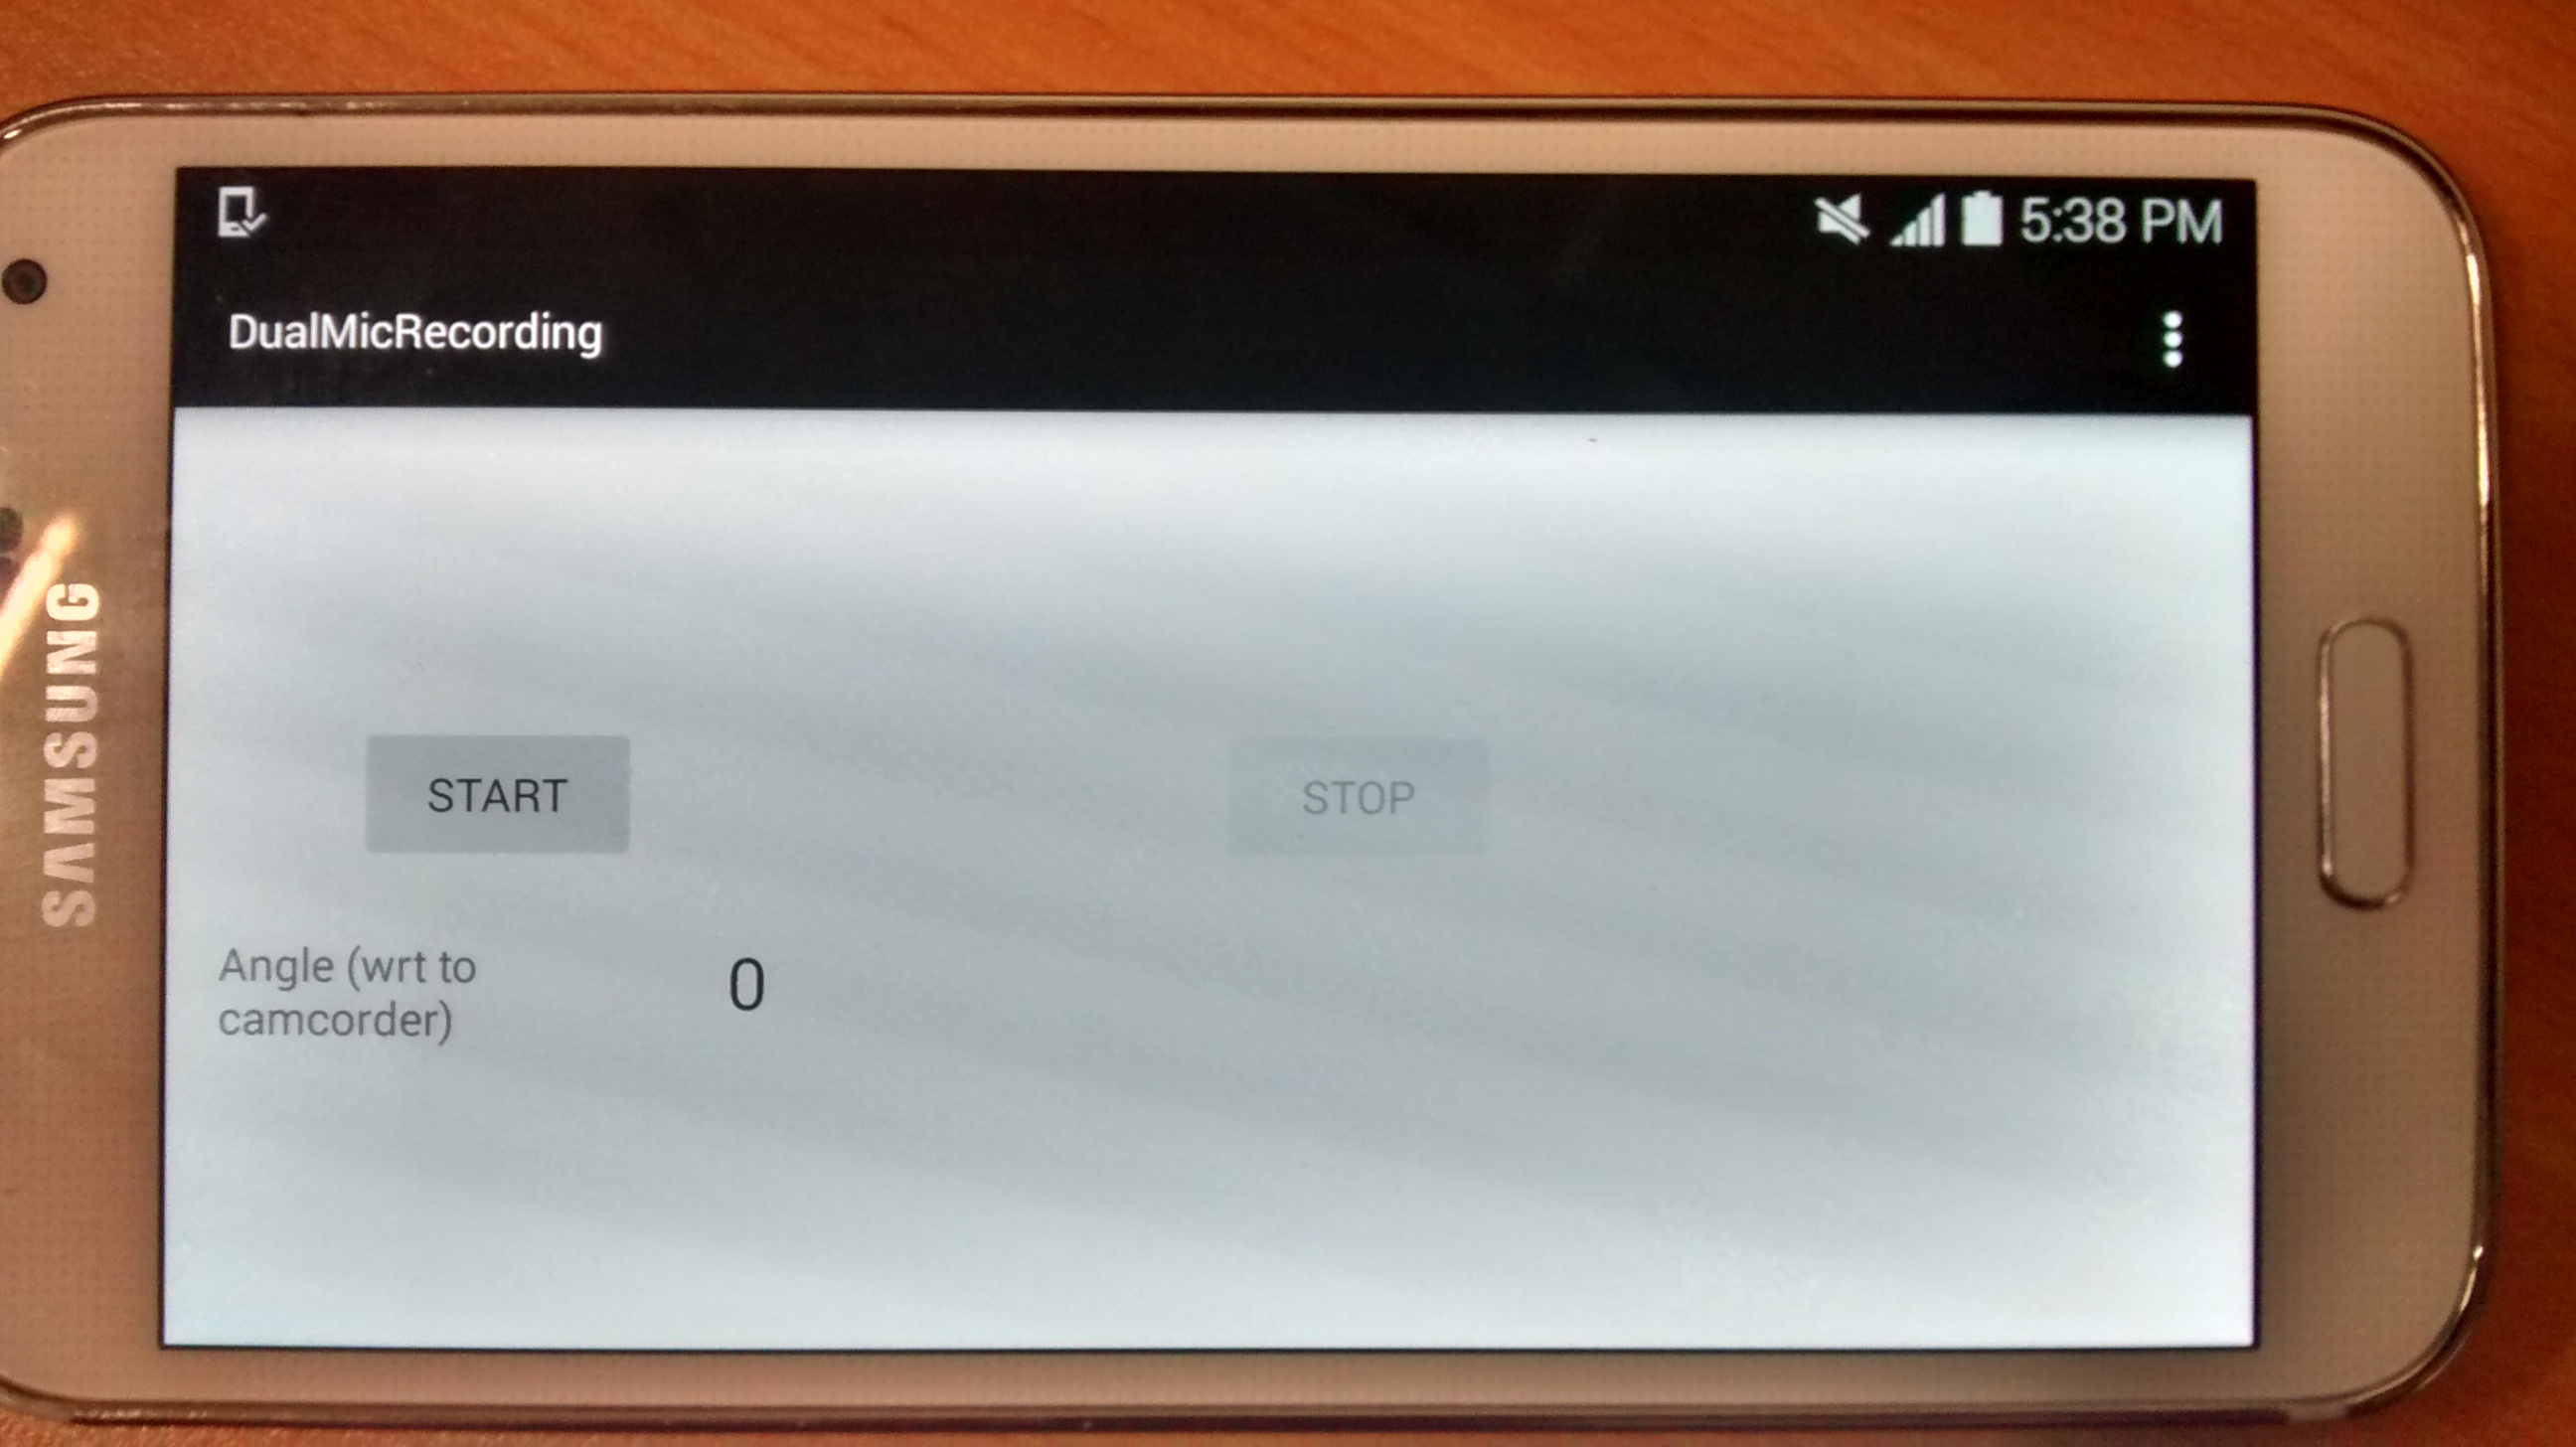
\includegraphics[width=90mm, height=60mm]{figures/screenshot.jpg}
\caption{Android Application Screenshot}
\label{fig:screenshot}
\end{figure}


\begin{figure}
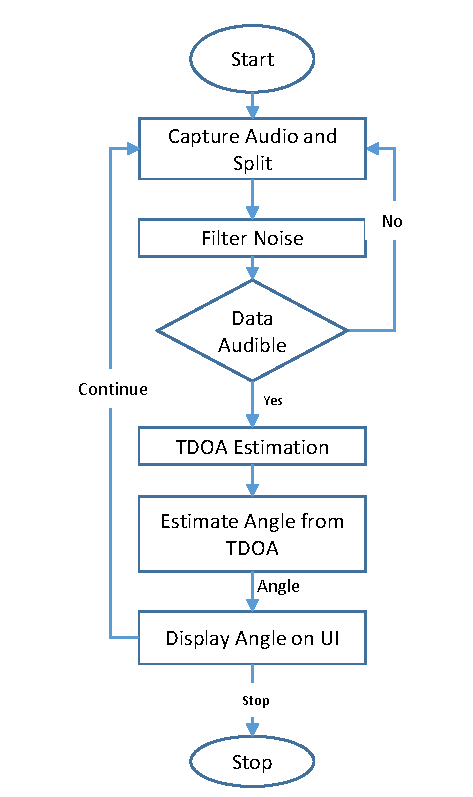
\includegraphics[width=80mm, height=100mm]{figures/flowchart.pdf}
%\includesvg{figures/flow_chart.svg}
\caption{Flow Chart of Angle Estimation}
\label{fig:flowChart}
\end{figure}

The flow chart in Figure ~\ref{flowChart} represents the steps of angle estimation. Once the user starts the detection process, by clicking on start button on application interface, the application start capturing sound samples from both the microphones i.e. camcorder and mic. The sampling rate can be varied from 8000 HZ to 44100 HZ. For our experiments, we used 44100 HZ because Android guarantees to support this sampling rate at all devices and also using higher frequency provides a better estimate. Each step of flow chart is explained below.
\subsection{Capture \& Separate Samples }
When recording audio in stereo mode, Android puts captured audio frames from both the microphones in one single buffer. For processing, the application can read data from this system buffer. In our analysis we read 4096 samples from this buffer. The samples at even indexes represents a different channel than the samples at odd indexes. Before proceeding further, we split this array into two different arrays, one for camcorder data and other for the mic data. Elements of these arrays are called frames of audio data. Individual frames are processed for angle estimation. 

\subsection{Noise filter}
Since the environment may have some noises, so before estimating angle for captured samples, we filter the possible noise. We compute root mean square value of sound magnitude. If this magnitude is lower than a certain threshold, 680 [reasons for selecting this]for our experiments, then these samples are not used for angle estimation and rather discarded. Also, some smartphones might have an inbuilt noise suppressor module, so on devices with that capability, we use noise suppressor module together with our noise filter.

\subsection{TDOA estimation}
The objective of this step is to find difference in time-of-arrival (TDOA) of both signals. The time difference might arise because microphones might be at different distances from the sound source. We use signal convolution for lag estimation. The idea behind this approach is that given two audio signal arrays, sum of their products will be maximum when both signals are similar. So, given camcorder and mic data array, we shift the frames of mic array and compute sum of products of frames of both arrays. Each shift represents a lag. For example, we start by left shifting elements of mic array by N. For this shift, sum of products of elements of camcorder and mic array is computed and  stored. This represents convolution value corresponding to lag equal to -N . This negative lag means that mic samples lag behind camcorder samples by N number of frames. Next, we compute convolution value for left shift equal to N-1 and store it. This process is carried on for N times for left shift followed by N times for right shift. We also compute sum of products for 0 lag.
From all these convolution values for different lags, we pick the maximum value and record the lag corresponding to that value. This lag value is actually lag in terms of number of frames, so we divide it with sampling frequency to calculate TDOA which represents difference in time-of-arrival in seconds.

\subsection{Compute angle from lag}
Once we have TDOA, we estimate angle of arrival from it. The angle of arrival derivation looks like as shown in Figure ~\ref{fig:aoaDerivation}. The sound source lies somewhere in first quadrant and the inclined straight lines represents sound waves coming from the source. Same technique is used for estimation when the sound source is in second quadrant as well. Here, d represents the distance between camcorder and mic of the smartphone, $d_T$ represents difference in distance traveled by both signals and $\theta$ represents the angle of arrival with respect to camcorder of the smartphone. Since, we already know TDOA, we can  $d_T$ using velocity of sound in air (343m/s). Since position of microphones may vary device to device, so we need to manually measure the distance between microphones. For our experiments, we used Samsung Galaxy S5 with value of d equals to 0.18 meters.

\begin{figure}
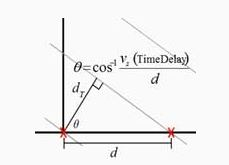
\includegraphics{figures/angle-of-arrival.jpg}
\caption{Angle of Arrival derivation ~\protect\cite{derivationSource}}
\label{fig:aoaDerivation}
\end{figure}

This approach can be used for angle estimation from 0 to 180 degrees only and hence the application wouldn't be able to differentiate sound sources in first and third quadrants with same TDOA values. Similarly, it is not feasible to differentiate between sources in second and fourth quadrants with same values of TDOA. We believe that if a smartphone has a third microphone (many high end smartphones have 3 microphones), then we can remove this limitation and then this same approach can be used to detect angles from 0 to 360 degress.

\subsection{Display angle on UI}
Once the angle is estimated, we display that on UI thread and continue estimating for next incoming samples. Angle computation and display occurs on two separate threads. The interface also displays a pointer corresponding to the angle for easier visualization of angle.
